\documentclass[12pt, a4paper]{article}
\usepackage{enumitem, amssymb }
\usepackage{fancyhdr}
\usepackage{graphicx}
\usepackage[english]{babel}
\usepackage{listings}
\usepackage{color}
\usepackage{fontspec} 

\lstset{basicstyle=\footnotesize\ttfamily,breaklines=true}
\lstset{framextopmargin=50pt,frame=bottomline}
\date{2020-6-16}
\author{Ebbe Vang}
\title{IDS Kit}
\pagestyle{fancy}
\fancyhf{}
\setlength{\headheight}{15pt}
\rhead{
\includegraphics[height=10pt]{RUC_BLACK_RGB.png}}
\lhead{Interactive Digital Systems}
\newlist{todolist}{itemize}{2}
\setlist[todolist]{label=$\square$}
\setmainfont{Arial}
\definecolor{mygreen}{rgb}{0,0.6,0}
\definecolor{mygray}{rgb}{0.5,0.5,0.5}
\definecolor{mymauve}{rgb}{0.58,0,0.82}

\lstset{ %
language=c++,
numbers=left,
backgroundcolor=\color{white},   % choose the background color
basicstyle=\footnotesize,        % size of fonts used for the code
breaklines=true,                 % automatic line breaking only at whitespace
captionpos=b,                    % sets the caption-position to bottom
commentstyle=\color{mygreen},    % comment style
escapeinside={\%*}{*)},          % if you want to add LaTeX within your code
keywordstyle=\color{blue},       % keyword style
stringstyle=\color{mymauve},     % string literal style
}

\begin{document}


\section{Content of the electronics kit}  

You borrow your kit personally from FlexLab and it must be handed back to
FlexLab at the end of the course.

When handing out, please check the contents with this list and
let us know if anything is missing. When handing in the kit, we also ask
you to check the contents and make us aware if you
have lost something or something is defective.
\begin{todolist}
  \item ESP32 Development Board
  \item 2 Breadboards (830 Point Solderless and Transparent)
  \item 2 Joysticks
  \item Potentiometer with cap
  \item GY-521 Accelerometer 
  \item Character LCD /w IIC/I2C Serial Interface Adapter
  \item 0.91inch OLED LCD Display Module 128x32 I2C 
  \item Micro USB Cable
  \item 3 push buttons
  \item Piezo Electronic Buzzer Alarm 95DB
  \item Small Toggle Switch Interruptor
  \item Cable Bundle
  \item various colored LEDs
  \item resistor
  \item RGB LED
\end{todolist}

%\section{about the Esp32 microcontroller}  

%\subsection{GPIO pins}

%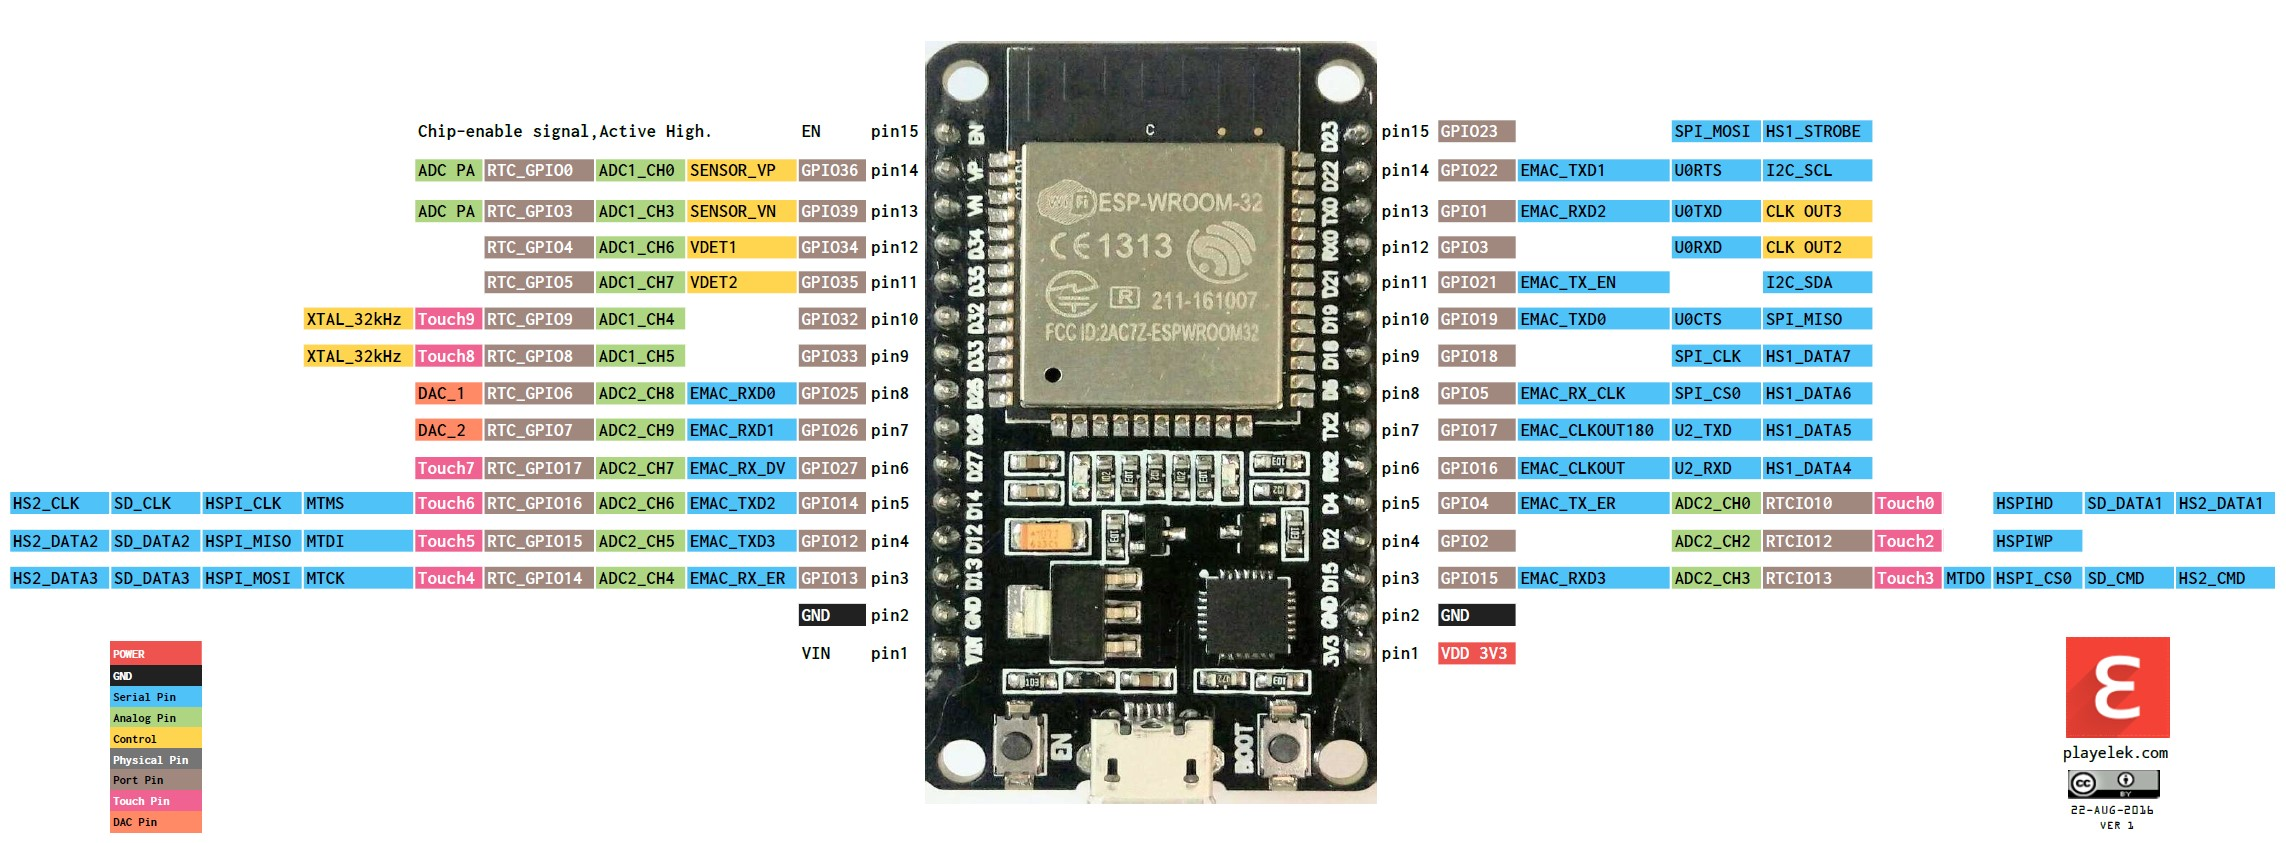
\includegraphics[width=\textwidth,keepaspectratio=true]{ESP32Espresiffboards12.jpg}

\newpage
\section{Code Examples}

\subsection{Digital Input}

In these first examples, we try to keep things simple and concentrate on controlling a single pin (LED) in the first example and then reading a pin (button) 
in the next example. In these examples we use digital input / output. 
Either there is power on the stick or there is not. 
Later in the next section we try with analog inputs and outputs, such as reading the resistance in a potentiometer or being able to control the brightness of an LED.

\subsubsection{Blink example}
The Blink example can be described as the "hello world"-script for microprocessors. Pay attention to the first line where we include arduino, this line of code is only necessary because we use platoformIO as our editor. If you search the net for blink or other arduino examples you will often find examples where this line is missing. That is because the arduino IDE add that by itself.


\lstinputlisting{code_examples/lecture_1/led.cpp}

\subsubsection{Button Example using 'Pullup'}

This example demonstration the use og a built in pullup resistor. 
The reason we use it the pullup resistor is to avoid that the voltage is fluctiating when the button isn't connected to the ground(gnd)
\lstinputlisting{code_examples/lecture_1/button.cpp}
\end{document}